\documentclass[11pt]{article}
\usepackage[margin=1in]{geometry}
\usepackage{amsmath,amssymb}
\usepackage{graphicx}
\usepackage{booktabs}
\usepackage{enumitem}
\usepackage{float}
\usepackage{caption}
\usepackage{xcolor}
\usepackage[colorlinks=true,linkcolor=black,urlcolor=blue]{hyperref}
\setlength{\parskip}{5pt}
\setlength{\parindent}{0pt}
\captionsetup{font=small,labelfont=bf}
\emergencystretch=3em

\title{\textbf{Project 2: Simple and Multiple Linear Regression}\\[2pt]
\large CS 4033/5033 Machine Learning Fundamentals, Fall 2026}
\author{Muhammad Ridwanul Hoque}
\date{}

\begin{document}
\maketitle

\begin{abstract}
I fit an ordinary least squares (OLS) linear regression model to each of nine synthetic datasets, which cover one, two and three predictors at low, moderate and high output noise. The regression code is written from scratch in NumPy, using a QR decomposition, and agrees with two independent solvers to within $3\times10^{-15}$. Every coefficient in every model is significant at the 1\% level, and the residual checks show no evidence against the linear model assumptions. The main finding is that the two usual metrics answer different questions. RMSE settles at a floor set by the noise (about 0.051, 0.113 and 0.135 for the three noise levels) and barely moves when predictors are added. $R^2$, in contrast, falls sharply with noise (from about 0.90 to 0.30 with one predictor) and rises with each added predictor (from 0.30 to 0.46 at high noise), because each new predictor contributes real signal. Ten-fold cross-validation confirms that none of the nine models overfits: out-of-sample RMSE is only 1.5\% to 4.6\% above the training RMSE, matching what theory predicts for $n = 100$.
\end{abstract}

\tableofcontents
\newpage

%=====================================================================
\section{Data}

The nine datasets each contain 100 data items. The files were supplied as PDF printouts of the comma-separated tables, so I converted each one to a CSV file by extracting the text and checking that every file has exactly 100 rows with the expected number of columns (2, 3 or 4). The values were not changed; files were renamed \texttt{1D\_L.csv}, \texttt{2D\_M.csv} and so on to remove spaces.

Before modeling, I checked a few properties of the inputs, because they affect how the results should be read.

\begin{itemize}[leftmargin=1.4em]
\item \textbf{All inputs lie in $[0, 1]$.} Every predictor ranges from about 0.007 to 0.994, so the coefficients are directly comparable in size.
\item \textbf{The inputs are shared across files.} The $x_1$ column is identical in all nine files, and $x_2$ is identical in the 2D and 3D files. Only $y$ changes.
\item \textbf{The inputs are close to uncorrelated.} In the 3D files, the pairwise correlations are $r_{12} = 0.052$, $r_{13} = 0.104$ and $r_{23} = 0.058$. This means adding a predictor should barely change the coefficients of the predictors already in the model, which turns out to be the case (Section~\ref{sec:combination}).
\item \textbf{The noise realization is shared across dimensions.} After fitting, the residuals of datasets with the same noise level are almost perfectly correlated across dimensions (correlation at least 0.982 for every pair, for example 1D Low against 2D Low). The generator appears to have reused the same noise draw for each noise level. This is useful: comparisons across 1, 2 and 3 predictors at a fixed noise level behave like a controlled experiment, in which only the number of predictors changes.
\end{itemize}

Figures~\ref{fig:data1d}, \ref{fig:data2d} and \ref{fig:data3d} show the raw data.

\begin{figure}[H]\centering
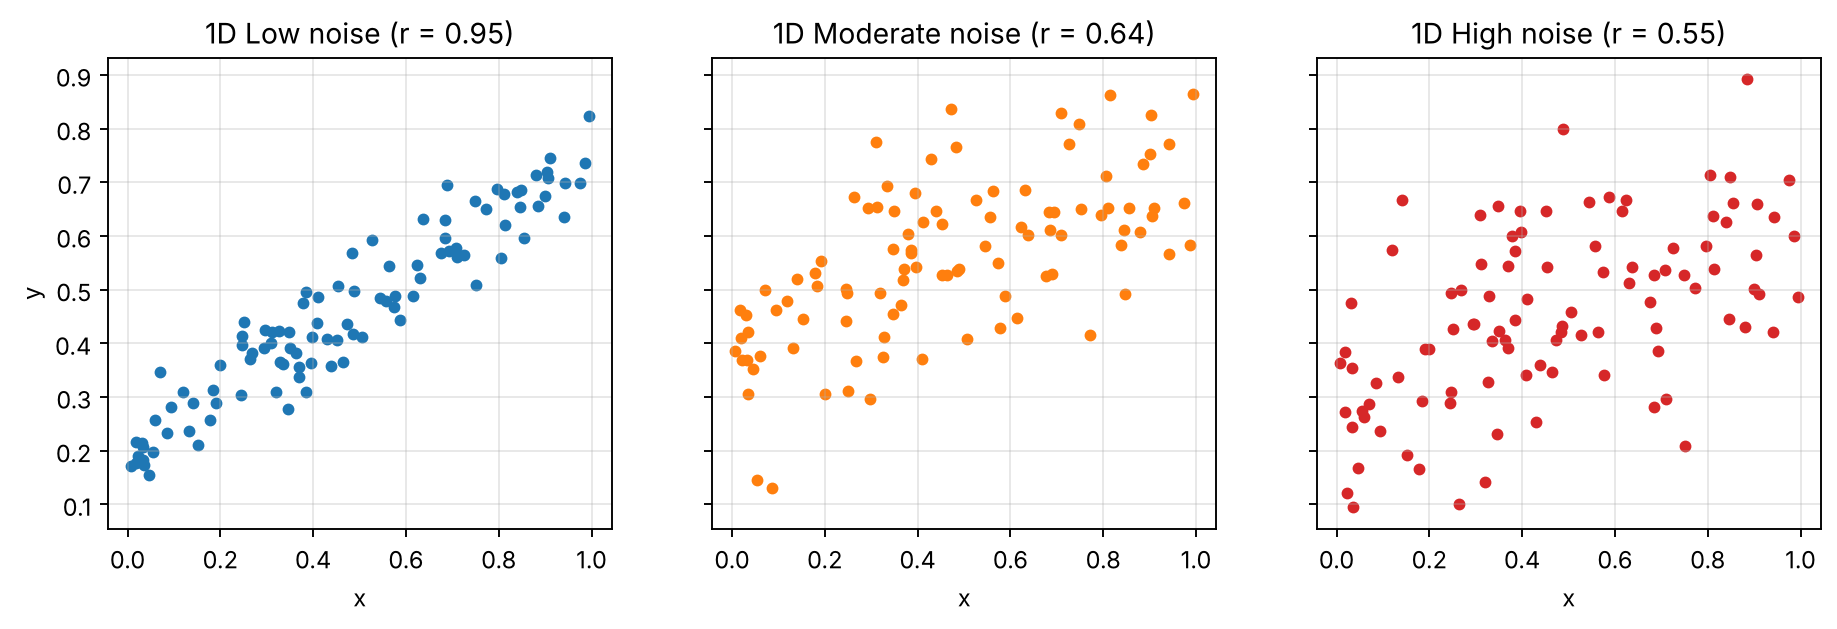
\includegraphics[width=\textwidth]{../figures/fig1_data_1d.png}
\caption{The three one-predictor datasets. The linear trend is obvious at low noise and much weaker at high noise. The title gives the Pearson correlation between $x$ and $y$.}
\label{fig:data1d}
\end{figure}

\begin{figure}[H]\centering
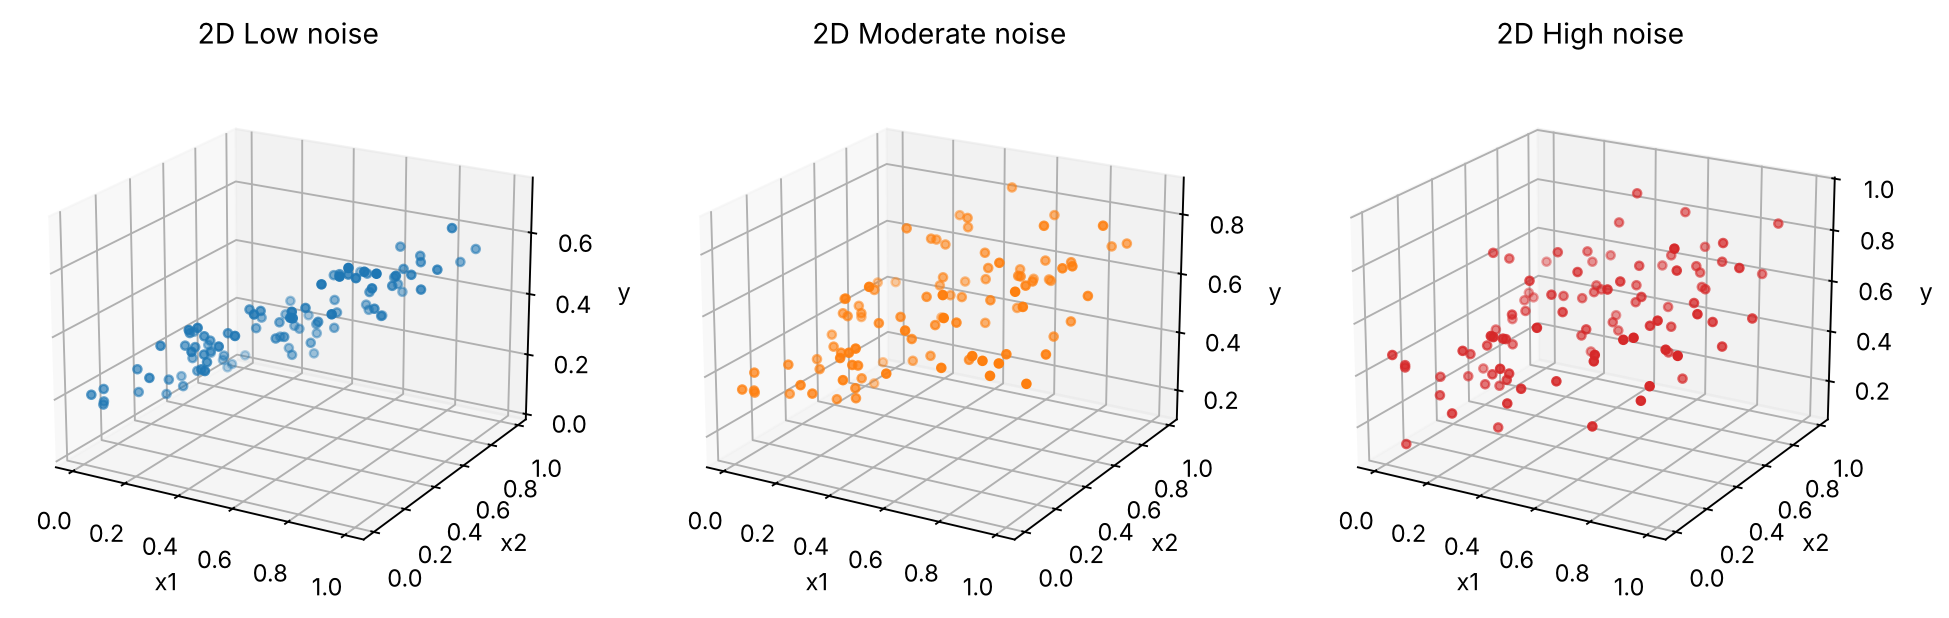
\includegraphics[width=\textwidth]{../figures/fig2_data_2d.png}
\caption{The three two-predictor datasets as 3D scatter plots of $(x_1, x_2, y)$.}
\label{fig:data2d}
\end{figure}

\begin{figure}[H]\centering
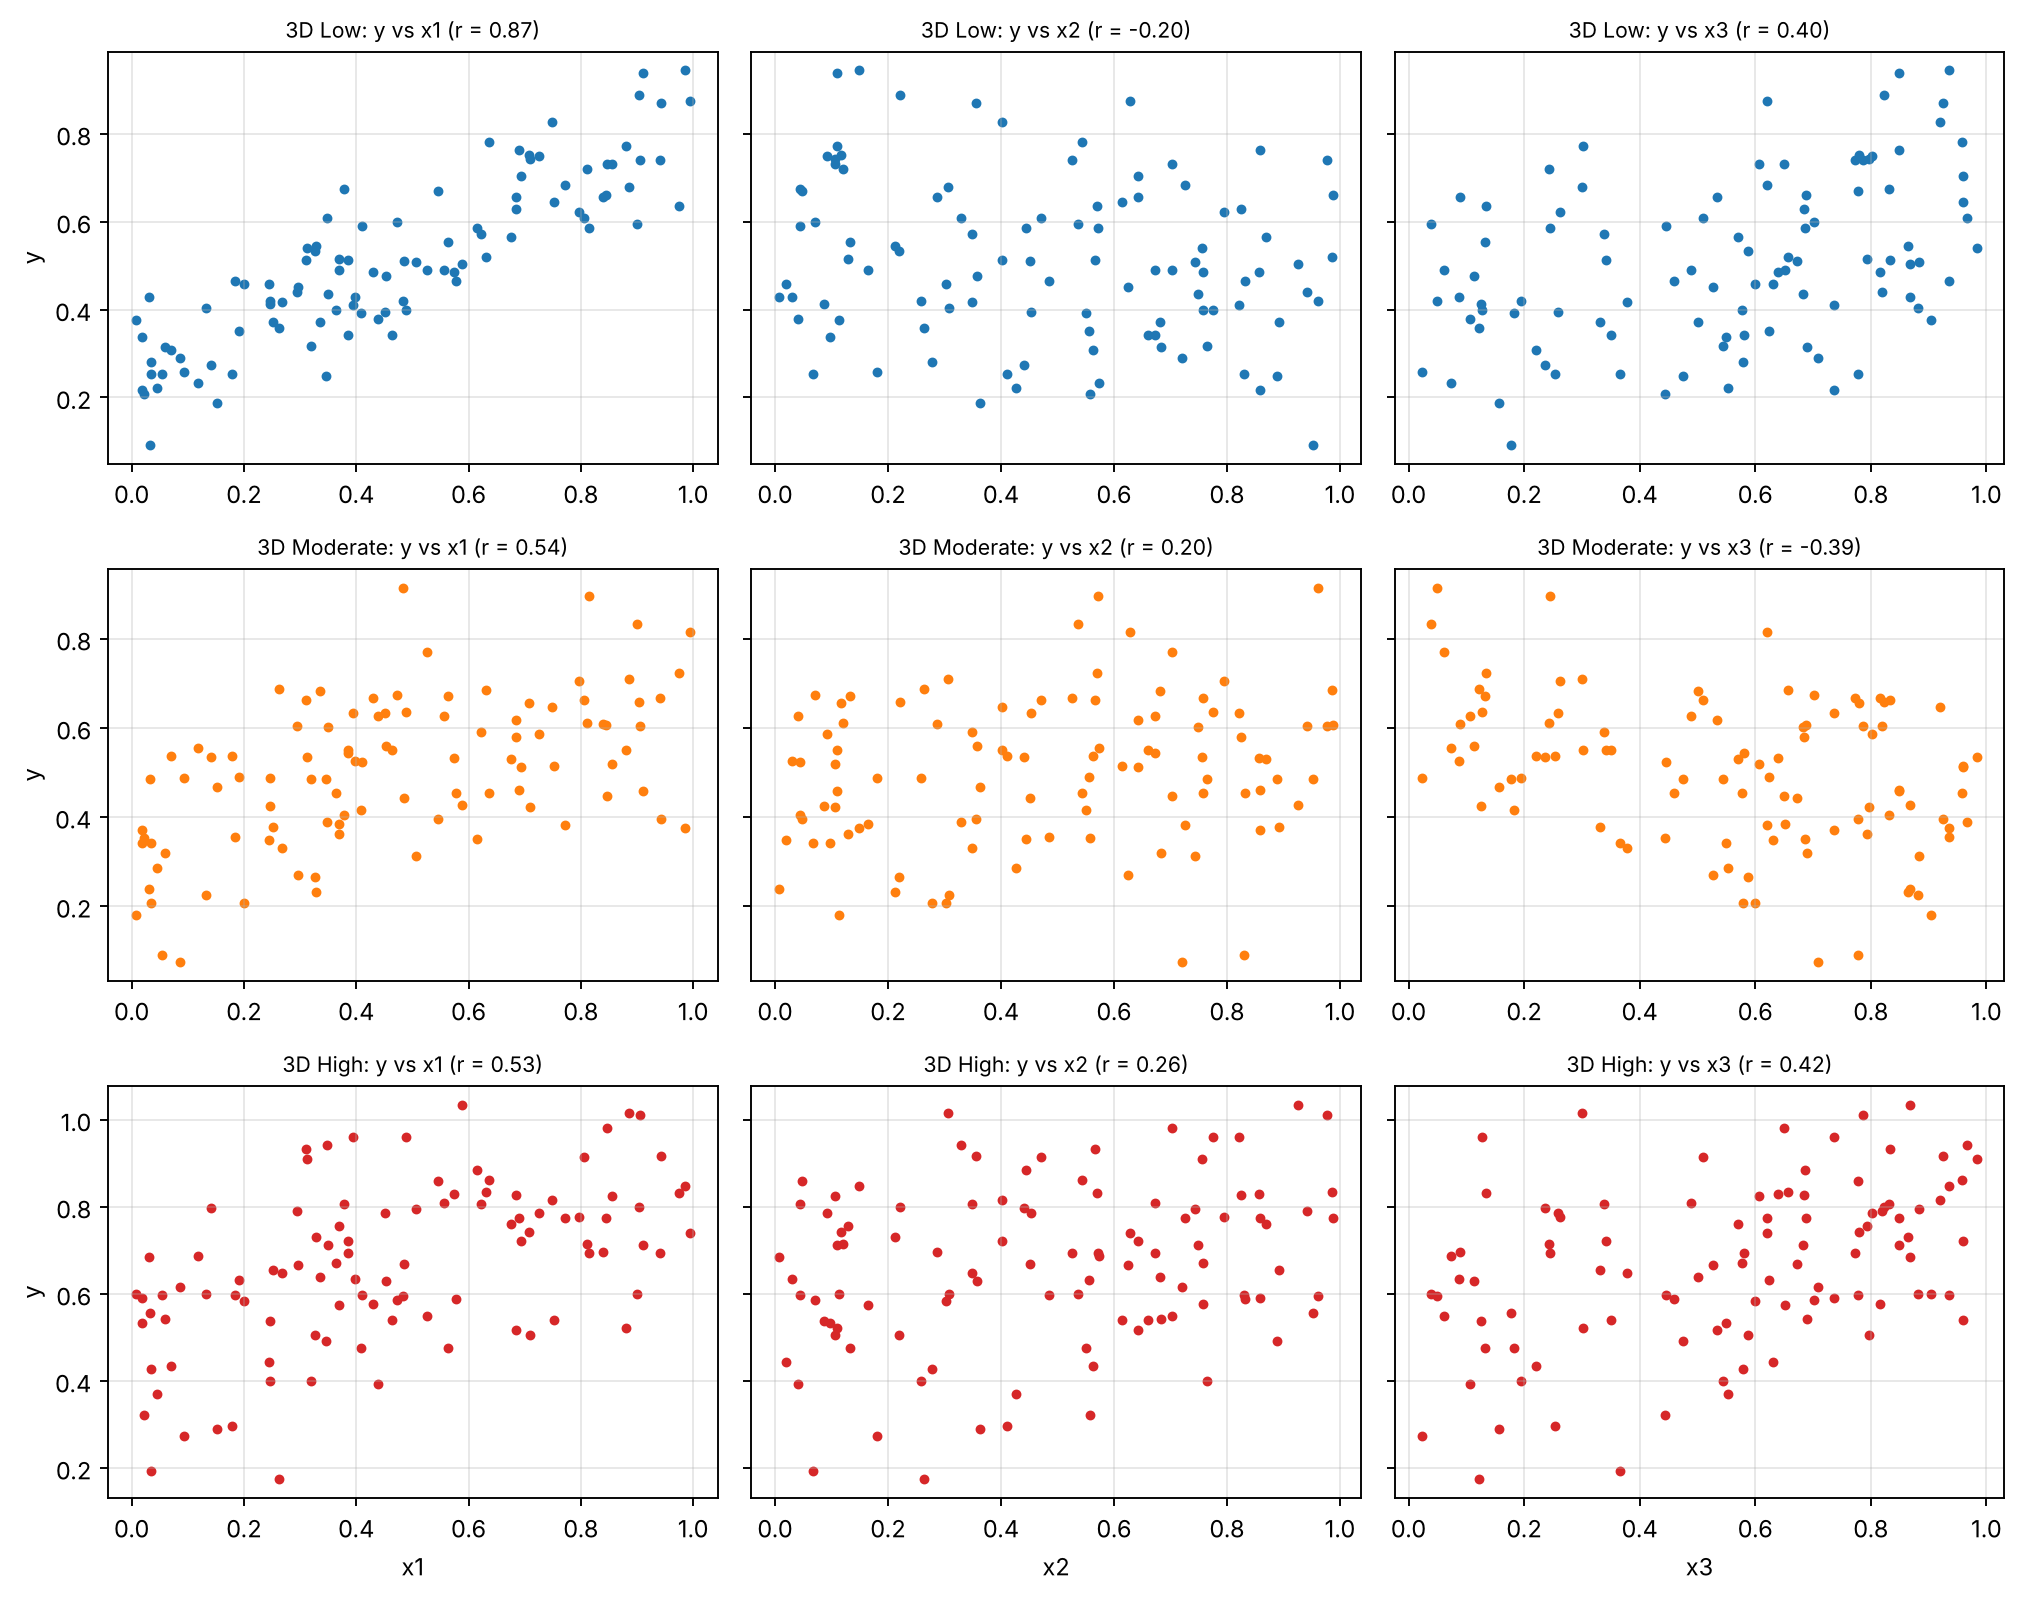
\includegraphics[width=0.92\textwidth]{../figures/fig3_data_3d.png}
\caption{The three-predictor datasets cannot be drawn in one picture, so each row shows $y$ against each predictor separately. Rows are noise levels. The marginal correlations hint at the sign and strength of each effect; for example $x_3$ has a negative effect in the Moderate file only.}
\label{fig:data3d}
\end{figure}

%=====================================================================
\section{Step 1: Form of the equation for each dataset}

Each dataset is modeled as a linear function of its predictors plus random error. With $\varepsilon$ denoting zero-mean Gaussian noise of constant variance $\sigma^2$, independent across data items, the forms are:

\begin{center}
\begin{tabular}{lll}
\toprule
Datasets & Model & Parameters to estimate\\
\midrule
1D L, 1D M, 1D H & $y = \beta_0 + \beta_1 x + \varepsilon$ & $\beta_0, \beta_1, \sigma$\\
2D L, 2D M, 2D H & $y = \beta_0 + \beta_1 x_1 + \beta_2 x_2 + \varepsilon$ & $\beta_0, \beta_1, \beta_2, \sigma$\\
3D L, 3D M, 3D H & $y = \beta_0 + \beta_1 x_1 + \beta_2 x_2 + \beta_3 x_3 + \varepsilon$ & $\beta_0, \beta_1, \beta_2, \beta_3, \sigma$\\
\bottomrule
\end{tabular}
\end{center}

The first is simple linear regression; the other two are multiple linear regression with one dependent variable. In matrix form all three are $\mathbf{y} = X\boldsymbol\beta + \boldsymbol\varepsilon$, where $X$ is the $100 \times (p+1)$ design matrix whose first column is all ones. The OLS estimate minimizes the residual sum of squares,
\[
\hat{\boldsymbol\beta} = \arg\min_{\boldsymbol\beta} \sum_{i=1}^{n} \big(y_i - \beta_0 - \textstyle\sum_j \beta_j x_{ij}\big)^2 = (X^TX)^{-1}X^T\mathbf{y}.
\]
The assignment states that each file was generated from a linear equation with Gaussian noise on the output, so this model form matches the data generating process. I have not added interaction or polynomial terms; the residual plots in Section~\ref{sec:assumptions} support that choice.

%=====================================================================
\section{Step 2: Metrics and why I use them}

No single number captures regression quality, so I report a small set of metrics. Each answers a different question.

\begin{center}\small
\begin{tabular}{p{3.2cm}p{4.6cm}p{6.6cm}}
\toprule
Metric & Definition & Why it is useful here\\
\midrule
$R^2$ & $1 - \text{RSS}/\text{TSS}$ & The share of the variance of $y$ explained by the model. It is unit-free, so the nine datasets can be compared on one scale. Its weakness is that it can only rise when predictors are added, so it is reported together with the next two.\\
Adjusted $R^2$ & $1 - (1-R^2)\frac{n-1}{n-p-1}$ & Penalizes each extra predictor. If adjusted $R^2$ rises with $p$, the new predictor adds more than chance would.\\
RMSE & $\sqrt{\text{RSS}/n}$ & Typical size of a prediction error, in the units of $y$. Because the noise is added to $y$, RMSE is directly comparable with the noise level and shows how close each fit is to the best possible.\\
MAE & $\frac1n\sum|y_i - \hat y_i|$ & Typical absolute error. Less sensitive to a few large residuals than RMSE; for Gaussian errors MAE $\approx 0.8\,$RMSE, which is a simple check.\\
$\hat\sigma$ (residual standard error) & $\sqrt{\text{RSS}/(n-p-1)}$ & Unbiased estimate of the noise standard deviation $\sigma$. It is the natural measure of each dataset's noise level.\\
Coefficient SE, $t$, $p$, 95\% CI & from $\hat\sigma^2 (X^TX)^{-1}$ & Tell us how precisely each $\beta_j$ is estimated and whether each predictor genuinely matters. This is essential for judging the fitted equations, not only the predictions.\\
Overall $F$ test & $\frac{(\text{TSS}-\text{RSS})/p}{\text{RSS}/(n-p-1)}$ & Tests whether the model as a whole beats predicting the mean of $y$.\\
10-fold CV RMSE and $R^2$ & out-of-fold predictions, repeated 10 times & All other metrics are computed on the data used for fitting. Cross-validation estimates performance on new data and reveals overfitting. Repeating it with 10 shuffles removes dependence on one split.\\
\bottomrule
\end{tabular}
\end{center}

I also run two diagnostic tests of the OLS assumptions, because the $p$-values and confidence intervals above are only valid if those assumptions hold: the Shapiro-Wilk test \cite{sw} for normality of the residuals, and the Breusch-Pagan test (Koenker's form) \cite{bp} for constant error variance.

%=====================================================================
\section{Step 3: Graphical representations and why I use them}

\begin{enumerate}[leftmargin=1.6em]
\item \textbf{Scatter plots of the raw data} (Figures~\ref{fig:data1d}, \ref{fig:data2d}, \ref{fig:data3d}). These show the strength of each trend and the noise level before any model is fit. For the 3D datasets, which cannot be drawn directly, I plot $y$ against each predictor separately.
\item \textbf{Regression line with data and residuals} for the 1D datasets (Figure~\ref{fig:fit1d}). This is the most direct check that a straight line is the right shape. The shaded band is the 95\% confidence interval for the mean response, which shows how well determined the line itself is.
\item \textbf{Regression plane with data and residuals} for the 2D datasets (Figure~\ref{fig:fit2d}). This is the two-predictor version of the line plot. Points above and below the plane are marked differently so that any systematic pattern would be visible.
\item \textbf{Predicted against actual values} for all nine datasets (Figure~\ref{fig:pva}). This works in any number of dimensions, so it is the main fit picture for the 3D datasets. A perfect model puts every point on the diagonal; scatter around it shows the error.
\item \textbf{Residuals against fitted values} (Figure~\ref{fig:resid}). This is the standard diagnostic for nonlinearity (a curved pattern) and non-constant variance (a funnel shape).
\item \textbf{Normal Q-Q plots of the residuals} (Figure~\ref{fig:qq}). These check the Gaussian error assumption that the confidence intervals and $p$-values rely on.
\item \textbf{Metric comparison chart} (Figure~\ref{fig:metrics}). $R^2$, RMSE and adjusted $R^2$ for all nine datasets, arranged by number of predictors and noise level, so the two main questions of the assignment can be read at a glance.
\item \textbf{Coefficient plot with 95\% confidence intervals} (Figure~\ref{fig:coefs}). This shows how precisely each coefficient is estimated and how that precision changes with noise.
\end{enumerate}

%=====================================================================
\section{Step 4: Regression software}

I wrote the regression code myself in Python with NumPy, in \texttt{src/linreg.py}. The class \texttt{OLSRegression} builds the design matrix with an intercept column and solves the least squares problem through a QR decomposition, $X = QR$, followed by the triangular solve $R\hat{\boldsymbol\beta} = Q^T\mathbf{y}$. This gives the same answer as the normal equations $(X^TX)^{-1}X^T\mathbf{y}$ but avoids forming $X^TX$, which squares the condition number and loses accuracy when predictors are nearly collinear. The same file computes every metric in Step 2, the coefficient covariance $\hat\sigma^2 R^{-1}R^{-T}$, the $F$ test, the Breusch-Pagan test and repeated $k$-fold cross-validation.

SciPy is used only for the $t$, $F$ and $\chi^2$ distribution functions that convert test statistics into $p$-values, and for the Shapiro-Wilk test. Matplotlib draws the figures. All of these are free and available to every OU student.

\textbf{Verification.} To make sure the implementation is correct, \texttt{src/verify.py} fits every dataset with two independent solvers: NumPy's SVD-based \texttt{np.linalg.lstsq} and scikit-learn's \texttt{LinearRegression}. Across the nine datasets the largest coefficient difference is $2.5\times10^{-16}$ against \texttt{lstsq} and $2.8\times10^{-15}$ against scikit-learn, and the largest $R^2$ difference is $1.1\times10^{-16}$. These are floating-point rounding differences, so the from-scratch code produces the same models as standard software. The full comparison is in \texttt{results/verification.csv}.

\textbf{How to run it.}
\begin{verbatim}
pip install numpy scipy matplotlib scikit-learn
cd src
python3 experiment.py    # fits all nine models, writes results/
python3 verify.py        # checks against lstsq and scikit-learn
python3 plots.py         # writes every figure to figures/
python3 make_tables.py   # writes the report tables
\end{verbatim}

%=====================================================================
\section{Step 5: Procedure}

For each of the nine datasets I fit one OLS model to all 100 data items and recorded the metrics in Step 2. OLS has no hyperparameters to tune, so no separate validation set is needed to choose a model. To estimate performance on unseen data, I ran 10-fold cross-validation repeated 10 times with different random shuffles (seed 0), refitting the model from scratch on each training fold. The results are written to \texttt{results/summary.csv} (one row per dataset), \texttt{results/coefficients.csv} (one row per coefficient) and \texttt{results/predictions/} (fitted value and residual for every data item).

%=====================================================================
\section{Step 6: Results, analysis and conclusions}

\subsection{The fitted equations}

Table~\ref{tab:eq} gives the equation found by regression for each dataset, with the standard error of each coefficient as a subscript. Every coefficient differs from zero at the 1\% level; the weakest are the $x_2$ coefficients in the Moderate and High files ($t \approx 2.8$, $p \approx 0.005$). The full inference table is in Appendix~\ref{app:coef}.

\begin{table}[H]\centering\small
\caption{Fitted regression equations. Subscripts are standard errors.}
\label{tab:eq}
\begin{tabular}{ll}
\toprule
Dataset & Fitted equation\\
\midrule
1D Low & $\hat y = 0.198_{(0.010)} + 0.549_{(0.018)}\,x$ \\
1D Moderate & $\hat y = 0.401_{(0.022)} + 0.332_{(0.040)}\,x$ \\
1D High & $\hat y = 0.308_{(0.026)} + 0.313_{(0.048)}\,x$ \\
\midrule
2D Low & $\hat y = 0.198_{(0.013)} + 0.549_{(0.019)}\,x_1 - 0.166_{(0.018)}\,x_2$ \\
2D Moderate & $\hat y = 0.327_{(0.028)} + 0.335_{(0.040)}\,x_1 + 0.111_{(0.039)}\,x_2$ \\
2D High & $\hat y = 0.323_{(0.034)} + 0.315_{(0.048)}\,x_1 + 0.134_{(0.047)}\,x_2$ \\
\midrule
3D Low & $\hat y = 0.214_{(0.016)} + 0.553_{(0.018)}\,x_1 - 0.165_{(0.018)}\,x_2 + 0.214_{(0.019)}\,x_3$ \\
3D Moderate & $\hat y = 0.436_{(0.034)} + 0.337_{(0.041)}\,x_1 + 0.112_{(0.039)}\,x_2 - 0.269_{(0.041)}\,x_3$ \\
3D High & $\hat y = 0.327_{(0.041)} + 0.316_{(0.049)}\,x_1 + 0.135_{(0.047)}\,x_2 + 0.232_{(0.049)}\,x_3$ \\

\bottomrule
\end{tabular}
\end{table}

\begin{table}[H]\centering\small
\caption{Fit metrics on all 100 data items. $\hat\sigma$ estimates the noise standard deviation.}
\label{tab:metrics}
\begin{tabular}{lccccccc}
\toprule
Dataset & $R^2$ & adj.\ $R^2$ & RMSE & MAE & $\hat\sigma$ & $F$ & $p(F)$\\
\midrule
1D Low & 0.901 & 0.900 & 0.0518 & 0.0427 & 0.0523 & 892.7 & 5.0e-51 \\
1D Moderate & 0.408 & 0.402 & 0.1136 & 0.0884 & 0.1148 & 67.6 & 8.4e-13 \\
1D High & 0.301 & 0.294 & 0.1357 & 0.1071 & 0.1371 & 42.3 & 3.3e-09 \\
\midrule
2D Low & 0.906 & 0.905 & 0.0518 & 0.0427 & 0.0526 & 470.1 & 1.2e-50 \\
2D Moderate & 0.452 & 0.441 & 0.1125 & 0.0870 & 0.1142 & 40.1 & 2.0e-13 \\
2D High & 0.352 & 0.338 & 0.1354 & 0.1067 & 0.1375 & 26.3 & 7.5e-10 \\
\midrule
3D Low & 0.924 & 0.922 & 0.0509 & 0.0413 & 0.0519 & 390.2 & 1.3e-53 \\
3D Moderate & 0.535 & 0.521 & 0.1123 & 0.0870 & 0.1146 & 36.9 & 6.2e-16 \\
3D High & 0.463 & 0.446 & 0.1354 & 0.1067 & 0.1382 & 27.6 & 6.1e-13 \\

\bottomrule
\end{tabular}
\end{table}

\begin{figure}[H]\centering
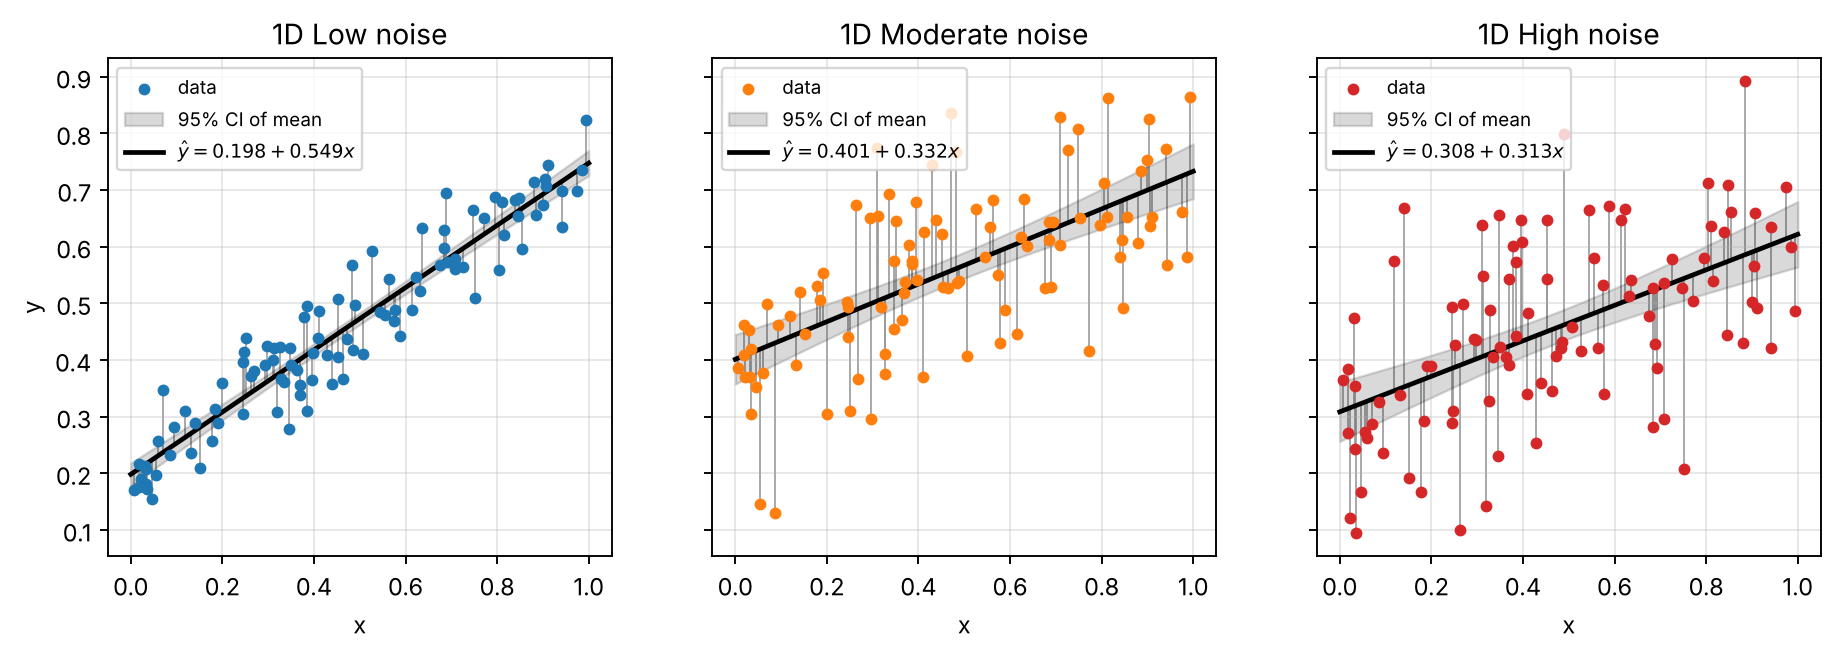
\includegraphics[width=\textwidth]{../figures/fig4_fit_1d.png}
\caption{Simple linear regression. Gray segments are residuals; the shaded band is the 95\% confidence interval for the mean of $y$ at each $x$.}
\label{fig:fit1d}
\end{figure}

\begin{figure}[H]\centering
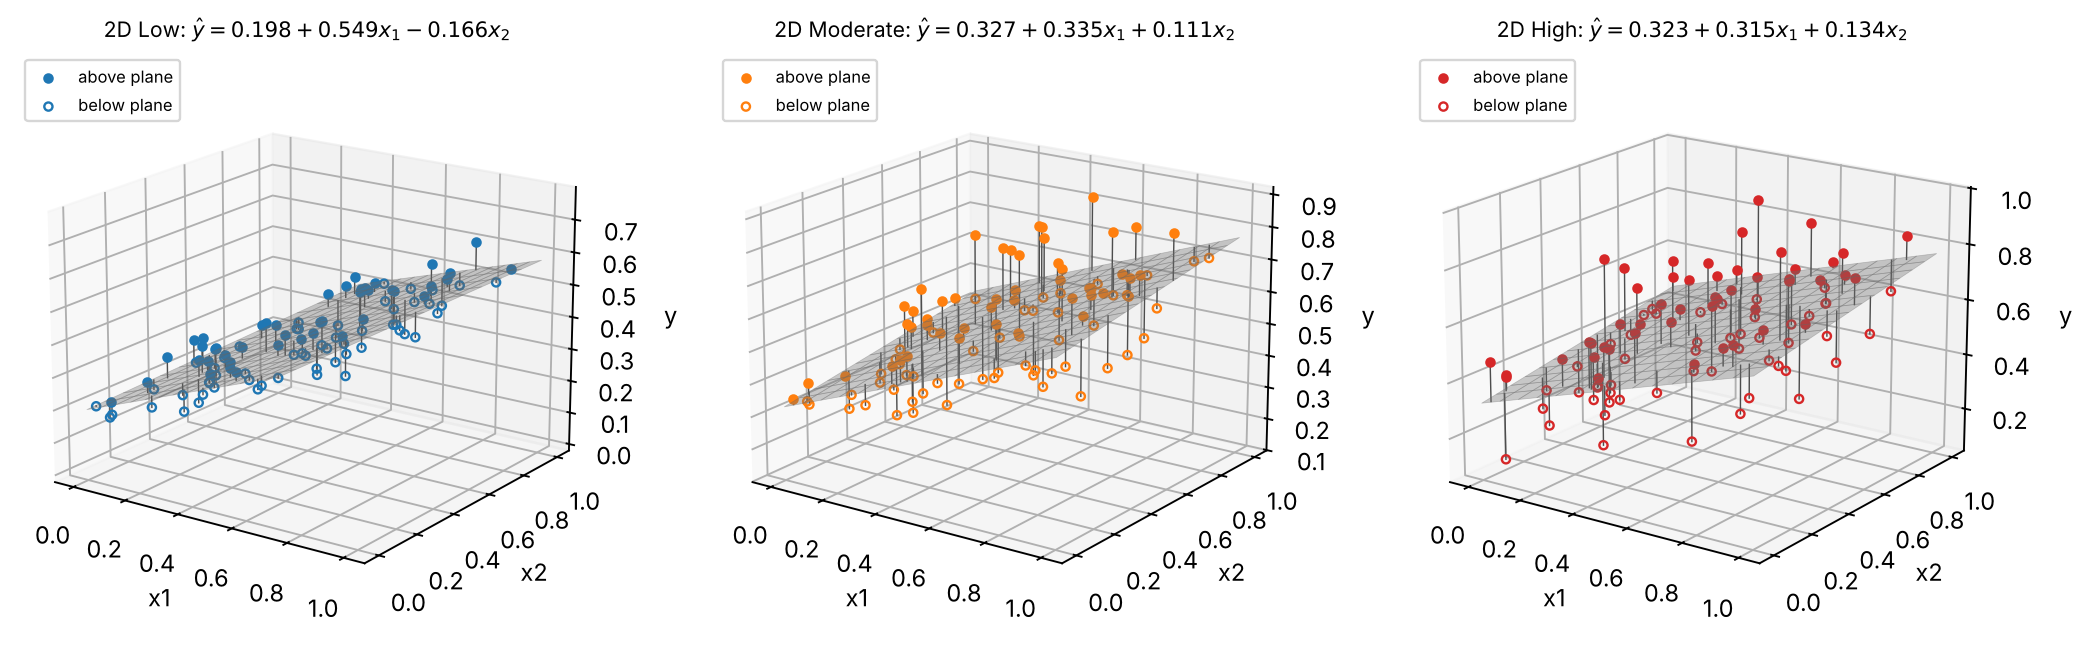
\includegraphics[width=\textwidth]{../figures/fig5_fit_2d.png}
\caption{Fitted regression planes for the two-predictor datasets. Filled points lie above the plane and hollow points below it; vertical segments are residuals.}
\label{fig:fit2d}
\end{figure}

\begin{figure}[H]\centering
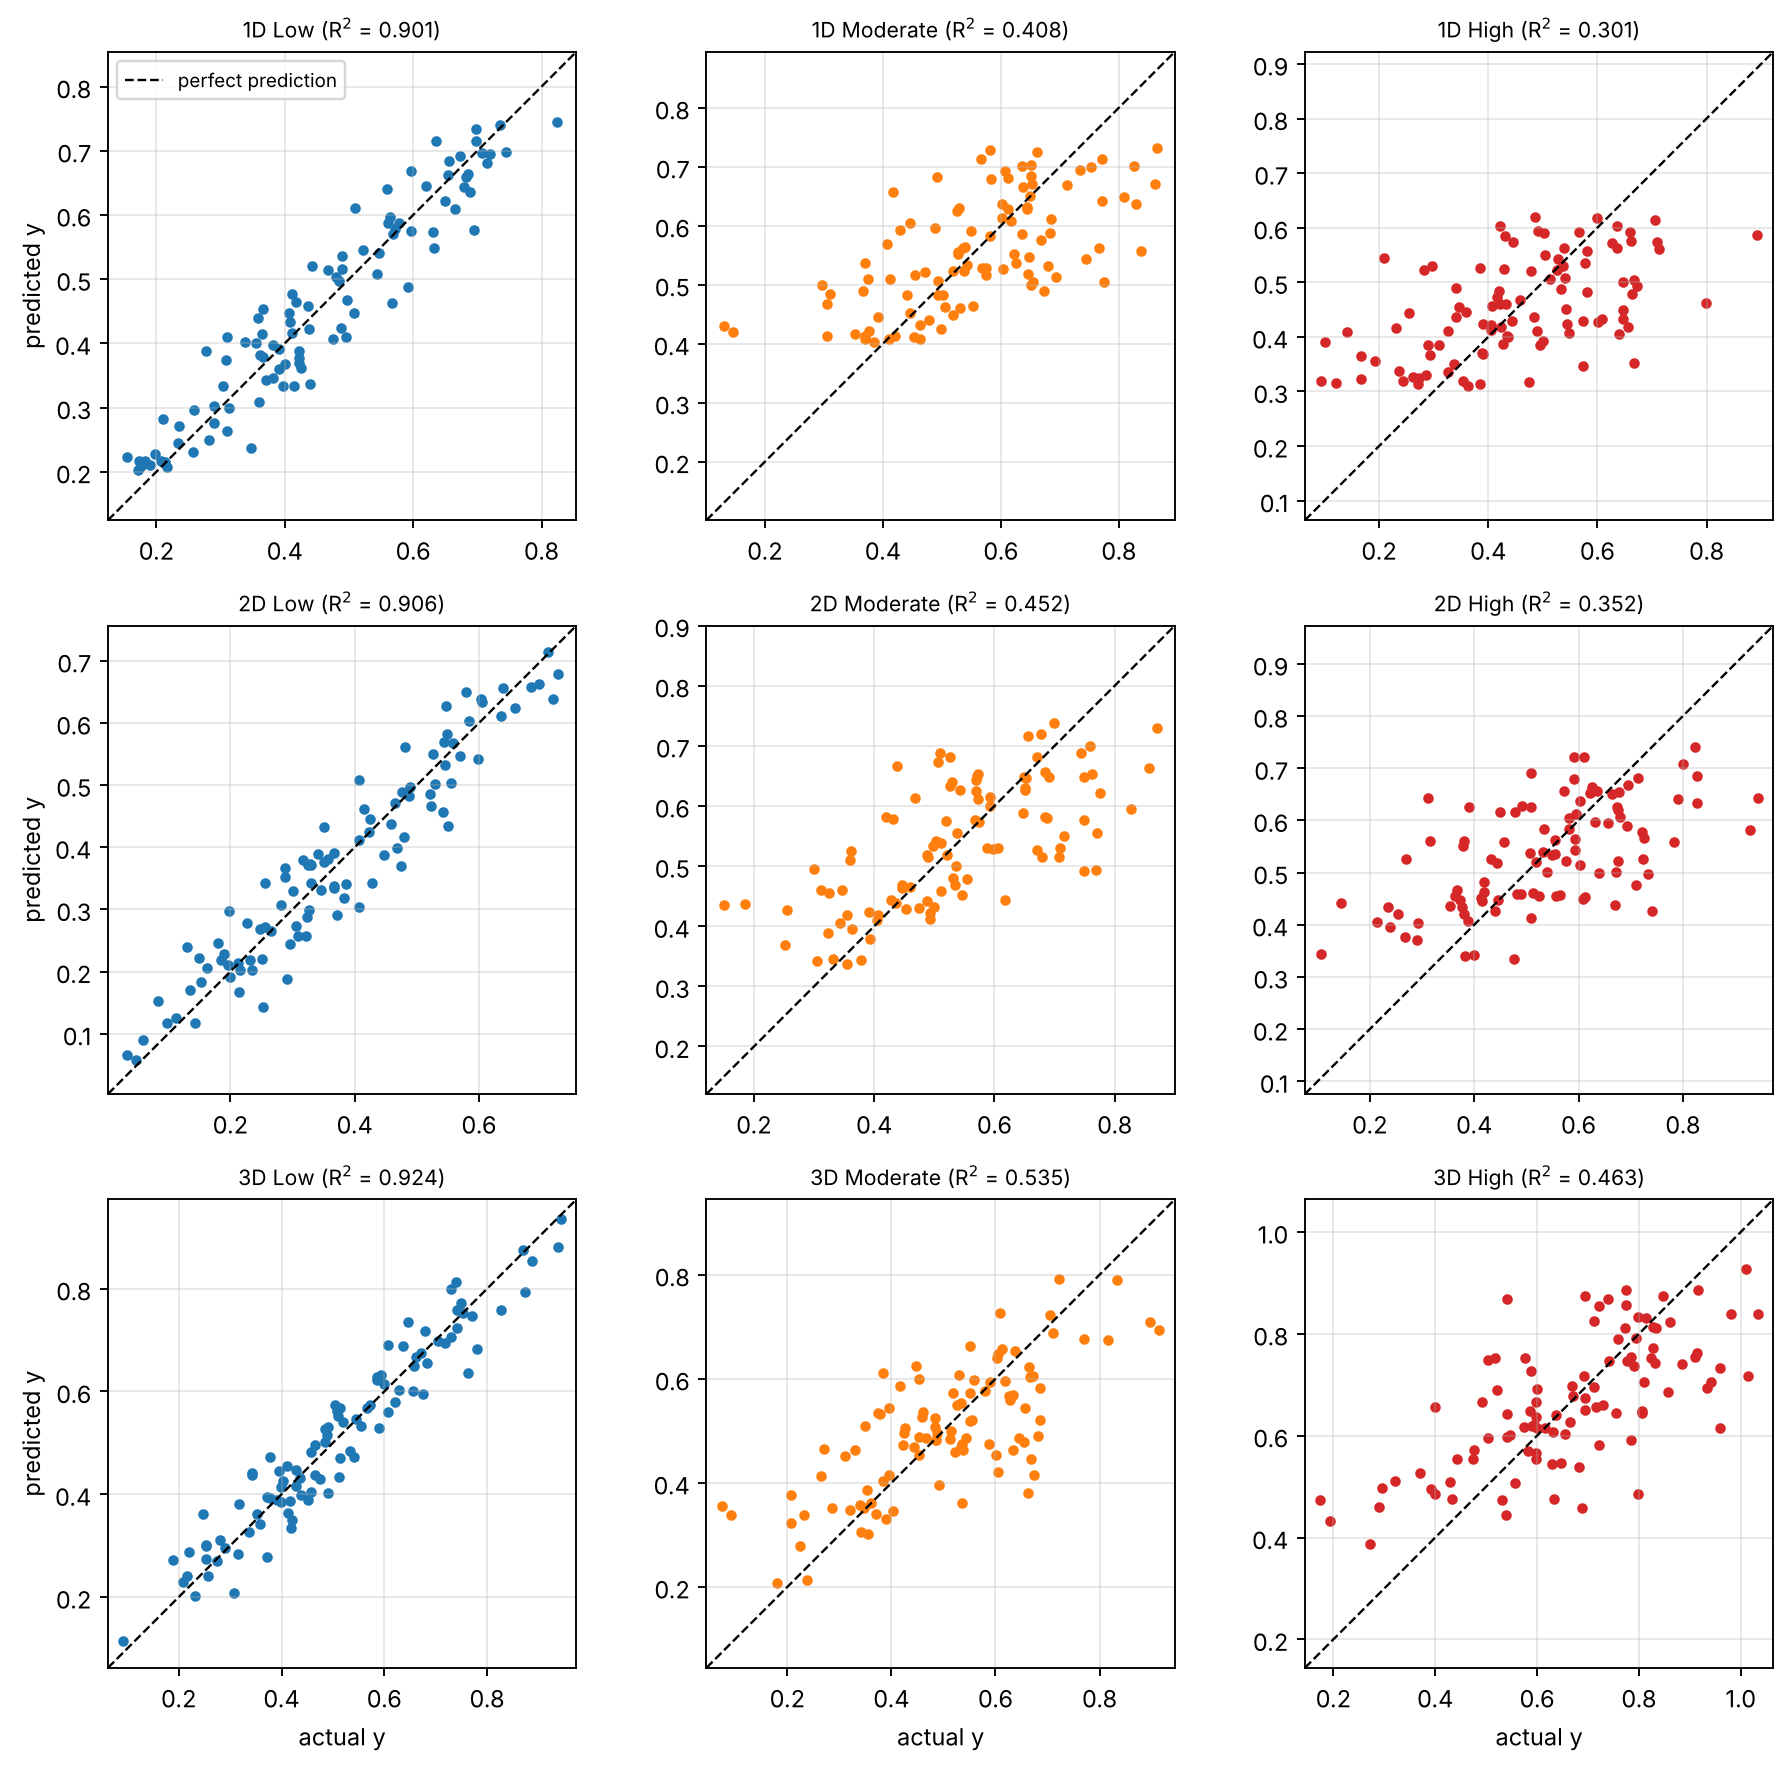
\includegraphics[width=0.84\textwidth]{../figures/fig6_pred_vs_actual.png}
\caption{Predicted against actual $y$ for all nine models. Rows are 1, 2 and 3 predictors; columns are noise levels. The dashed line is perfect prediction.}
\label{fig:pva}
\end{figure}

\subsection{Each dataset individually}

\textbf{One predictor.} At low noise the fitted line $\hat y = 0.198 + 0.549x$ explains 90.1\% of the variance and the data hug the line (Figure~\ref{fig:fit1d}). At moderate and high noise, the slope is still clearly significant ($t = 8.2$ and $6.5$) but the line explains only 40.8\% and 30.1\% of the variance. The confidence band also widens with noise, so the line itself is less certain. The 1D Moderate and 1D High lines have similar slopes (0.332 and 0.313) but different intercepts (0.401 and 0.308), so they come from different generating equations, not just different noise.

\textbf{Two predictors.} The regression planes (Figure~\ref{fig:fit2d}) tilt along both axes. At low noise, $x_2$ has a clear negative effect ($-0.166$, $t = -9.2$), while at moderate and high noise it has a smaller positive effect ($+0.111$ and $+0.134$). The low noise plane fits so closely that the residual segments are barely visible; at high noise the points scatter widely above and below the plane, with no sign of curvature or a pattern by region.

\textbf{Three predictors.} The predicted against actual plots (Figure~\ref{fig:pva}, bottom row) show a tight diagonal at low noise ($R^2 = 0.924$) and a loose cloud at high noise ($R^2 = 0.463$). The new predictor $x_3$ is significant in all three files, but its sign changes: $+0.214$ (Low), $-0.269$ (Moderate) and $+0.232$ (High). Without the regression, the marginal plots of Figure~\ref{fig:data3d} would make these effects hard to see at higher noise.

\subsection{Effect of increasing noise}

Noise is the dominant factor in every metric (Figure~\ref{fig:metrics}). Going from low to high noise with one predictor:
\begin{itemize}[leftmargin=1.4em]
\item $R^2$ falls from 0.901 to 0.301, and RMSE rises from 0.052 to 0.136, a factor of 2.6.
\item The estimated noise standard deviation $\hat\sigma$ is about 0.052, 0.114 and 0.137 for Low, Moderate and High, essentially the same at every dimension. RMSE sits right at this level in every model, which is the best a correctly specified model can do: once the true linear function is found, what remains is the noise, which no model of $x$ can predict.
\item Coefficient standard errors grow in proportion to $\hat\sigma$. For $\beta_1$ they are about 0.018, 0.040 and 0.048 (Figure~\ref{fig:coefs}), so the 95\% confidence interval for the slope widens from about $\pm 0.04$ to about $\pm 0.10$.
\item The step from Moderate to High is smaller than from Low to Moderate ($\hat\sigma$ grows by about 20\% against about 120\%), and the gap between the Moderate and High metrics is correspondingly smaller.
\end{itemize}

\subsection{Effect of increasing the number of predictors}
\label{sec:combination}

Because the inputs and the noise draw are shared across files, comparing 1, 2 and 3 predictors at the same noise level isolates the effect of the extra predictors.

\begin{itemize}[leftmargin=1.4em]
\item \textbf{RMSE does not change.} At each noise level, RMSE stays the same to within about 0.001 across one, two and three predictors (Table~\ref{tab:metrics}). The error cannot fall below the noise, and each model already reaches it.
\item \textbf{$R^2$ rises.} At high noise $R^2$ goes from 0.301 to 0.352 to 0.463. This is not overfitting. Each added predictor carries real signal, so the variance of $y$ grows (its standard deviation goes from 0.162 to 0.168 to 0.185 at high noise) while the unexplained noise stays fixed. A larger share of the variance is therefore explained. Adjusted $R^2$ and cross-validated $R^2$ rise as well, which confirms the gain is genuine.
\item \textbf{The coefficients are stable.} Because the predictors are almost uncorrelated, adding $x_2$ or $x_3$ leaves the earlier coefficients nearly unchanged. For example, the $x_1$ coefficient at low noise is 0.549, 0.549 and 0.553 in the 1D, 2D and 3D models, and the $x_2$ coefficient at high noise is 0.134 and 0.135 in the 2D and 3D models. Its standard error barely changes either.
\item \textbf{Each predictor uses up one degree of freedom.} With $n = 100$ and at most $p = 3$ this costs very little, but the effect is visible in cross-validation: the gap between training and cross-validated RMSE grows from 1.5\% to 2.6\% to 3.8\% at low noise (Table~\ref{tab:cv}).
\end{itemize}

\begin{figure}[H]\centering
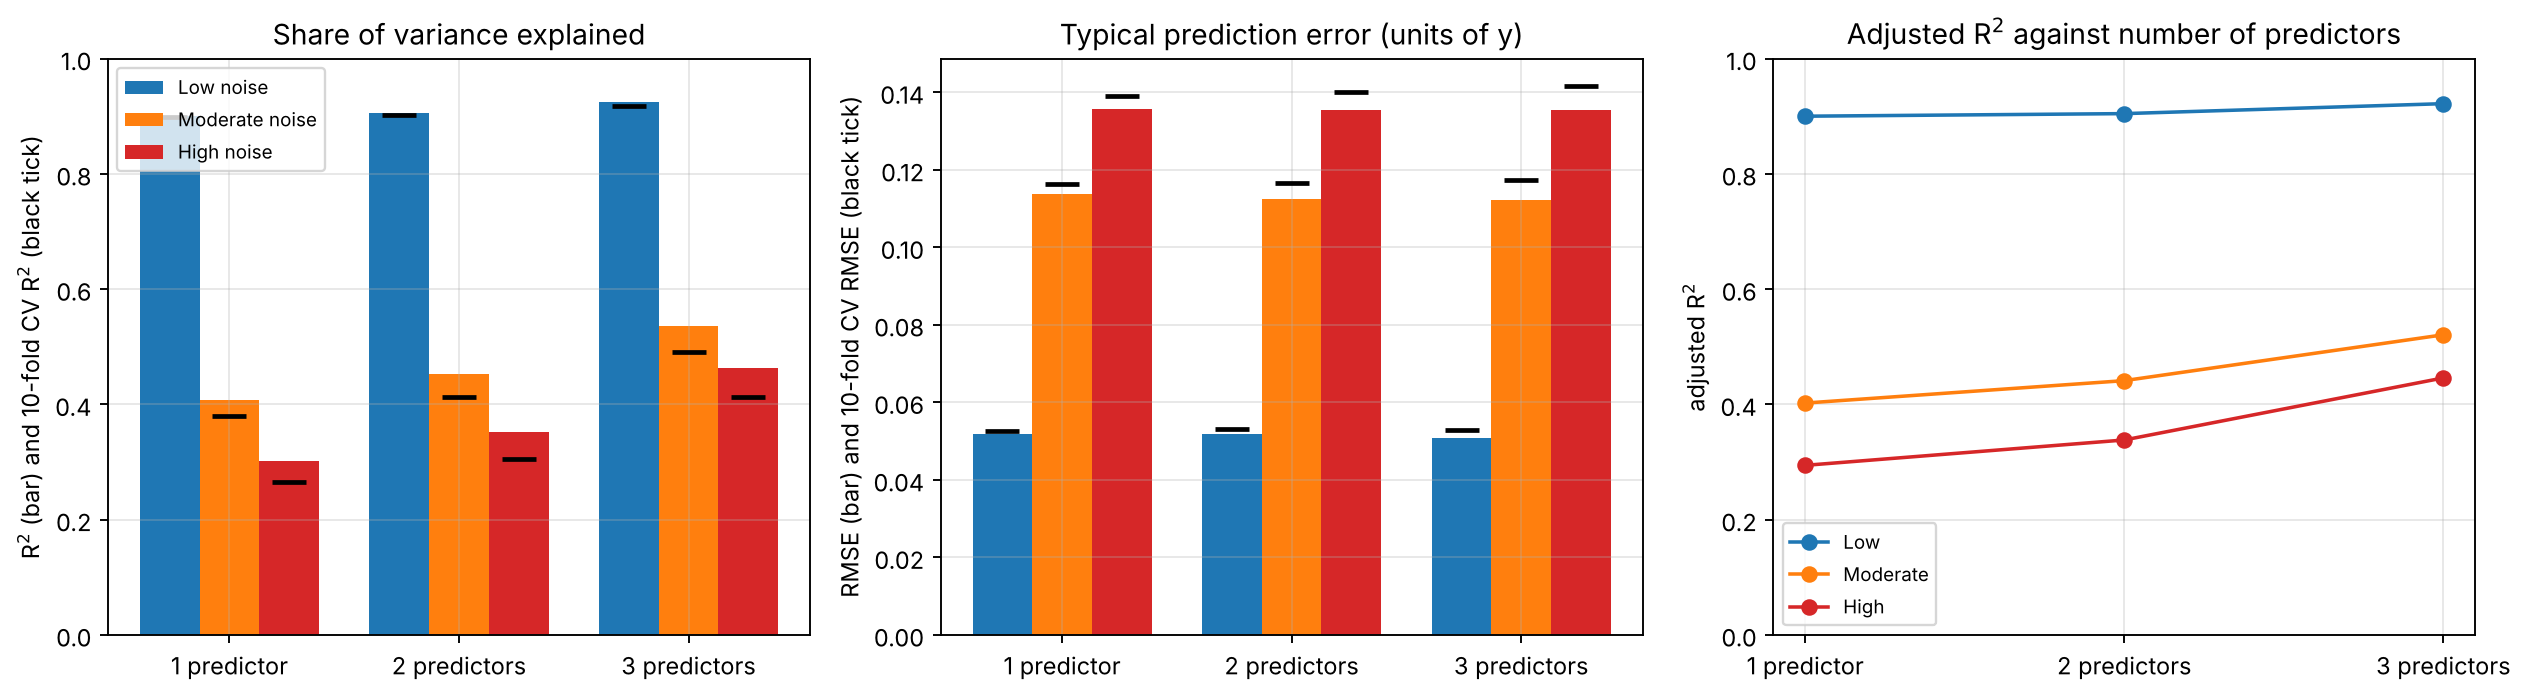
\includegraphics[width=\textwidth]{../figures/fig9_metrics.png}
\caption{Metrics by number of predictors and noise level. Black ticks mark the 10-fold cross-validated values. RMSE is flat across predictors, while $R^2$ and adjusted $R^2$ rise with each predictor.}
\label{fig:metrics}
\end{figure}

\begin{figure}[H]\centering
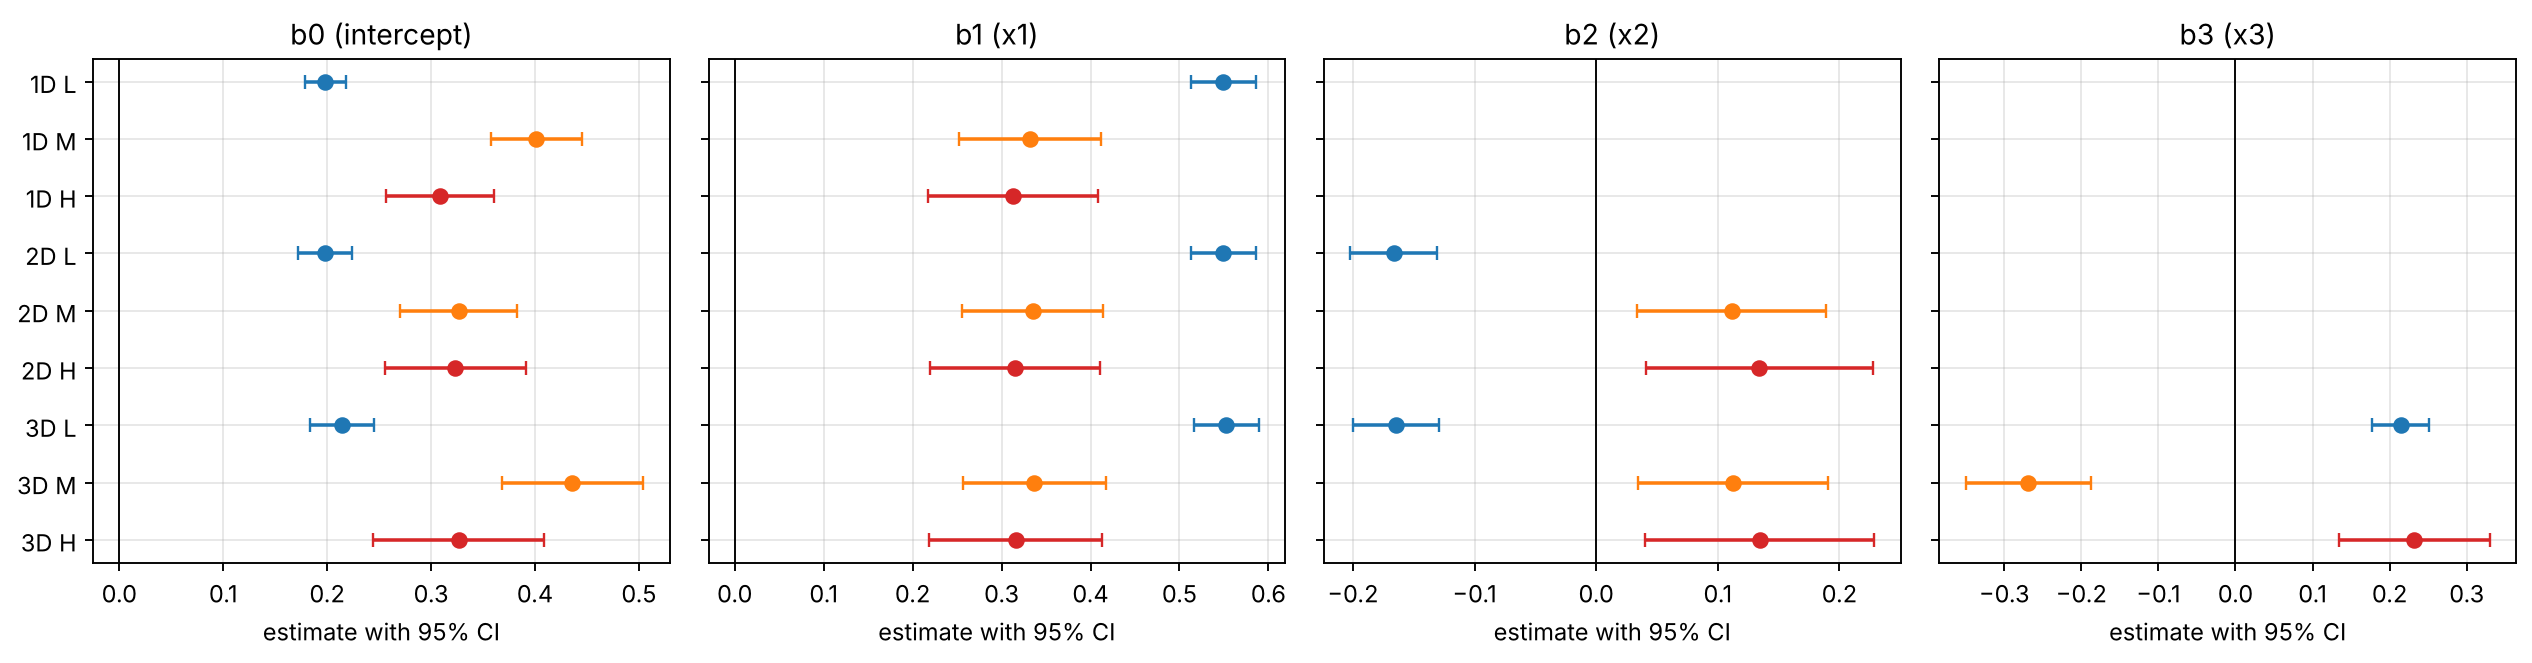
\includegraphics[width=\textwidth]{../figures/fig10_coefficients.png}
\caption{Every coefficient with its 95\% confidence interval. Intervals widen with noise, but none crosses zero.}
\label{fig:coefs}
\end{figure}

\subsection{Generalization}

Table~\ref{tab:cv} compares the training RMSE with the 10-fold cross-validated RMSE. For a correct linear model with $p$ predictors fit to $n$ items, theory predicts an expected out-of-sample RMSE of about $\hat\sigma\sqrt{1 + (p+1)/n}$ \cite{islr}. The cross-validated values agree with this prediction to within 0.001 in every case. The gap between training and cross-validated RMSE is small (1.5\% to 4.6\%) and grows with both the number of predictors and the noise level, as expected: more parameters, and noisier data, each make the fitted coefficients vary a little more from sample to sample. The models are therefore not overfitting, and the training metrics in Table~\ref{tab:metrics} are reliable descriptions of how the models would perform on new data from the same source.

\begin{table}[H]\centering\small
\caption{Training against 10-fold cross-validated performance (mean $\pm$ standard deviation over 10 repeats). ``Expected'' is $\hat\sigma\sqrt{1+(p+1)/n}$.}
\label{tab:cv}
\begin{tabular}{lcccccc}
\toprule
Dataset & RMSE & CV RMSE & Gap & Expected & $R^2$ & CV $R^2$\\
\midrule
1D Low & 0.0518 & 0.0526 $\pm$ 0.0003 & 1.5\% & 0.0528 & 0.901 & 0.898 \\
1D Moderate & 0.1136 & 0.1163 $\pm$ 0.0006 & 2.4\% & 0.1159 & 0.408 & 0.380 \\
1D High & 0.1357 & 0.1392 $\pm$ 0.0009 & 2.5\% & 0.1385 & 0.301 & 0.266 \\
\midrule
2D Low & 0.0518 & 0.0531 $\pm$ 0.0003 & 2.6\% & 0.0534 & 0.906 & 0.902 \\
2D Moderate & 0.1125 & 0.1165 $\pm$ 0.0007 & 3.6\% & 0.1159 & 0.452 & 0.413 \\
2D High & 0.1354 & 0.1400 $\pm$ 0.0010 & 3.4\% & 0.1395 & 0.352 & 0.306 \\
\midrule
3D Low & 0.0509 & 0.0528 $\pm$ 0.0003 & 3.8\% & 0.0529 & 0.924 & 0.918 \\
3D Moderate & 0.1123 & 0.1175 $\pm$ 0.0006 & 4.6\% & 0.1169 & 0.535 & 0.492 \\
3D High & 0.1354 & 0.1416 $\pm$ 0.0007 & 4.6\% & 0.1409 & 0.463 & 0.412 \\

\bottomrule
\end{tabular}
\end{table}

\subsection{Checking the model assumptions}
\label{sec:assumptions}

The residual plots (Figure~\ref{fig:resid}) show a horizontal band with no curvature and no funnel shape, which supports both the linear form and constant variance. About 95\% of the residuals fall inside $\pm 2\hat\sigma$, as expected for Gaussian errors. The Q-Q plots (Figure~\ref{fig:qq}) follow the reference line closely. The formal tests agree (Table~\ref{tab:assump}): no Shapiro-Wilk $p$-value is below 0.38, so there is no evidence against normal errors, and no Breusch-Pagan $p$-value is below 0.05, so there is no evidence of heteroscedasticity. The smallest Breusch-Pagan value (0.09, for 3D Moderate) is what we would expect to see now and then by chance among nine tests. The confidence intervals and $p$-values reported above can therefore be trusted.

\begin{figure}[H]\centering
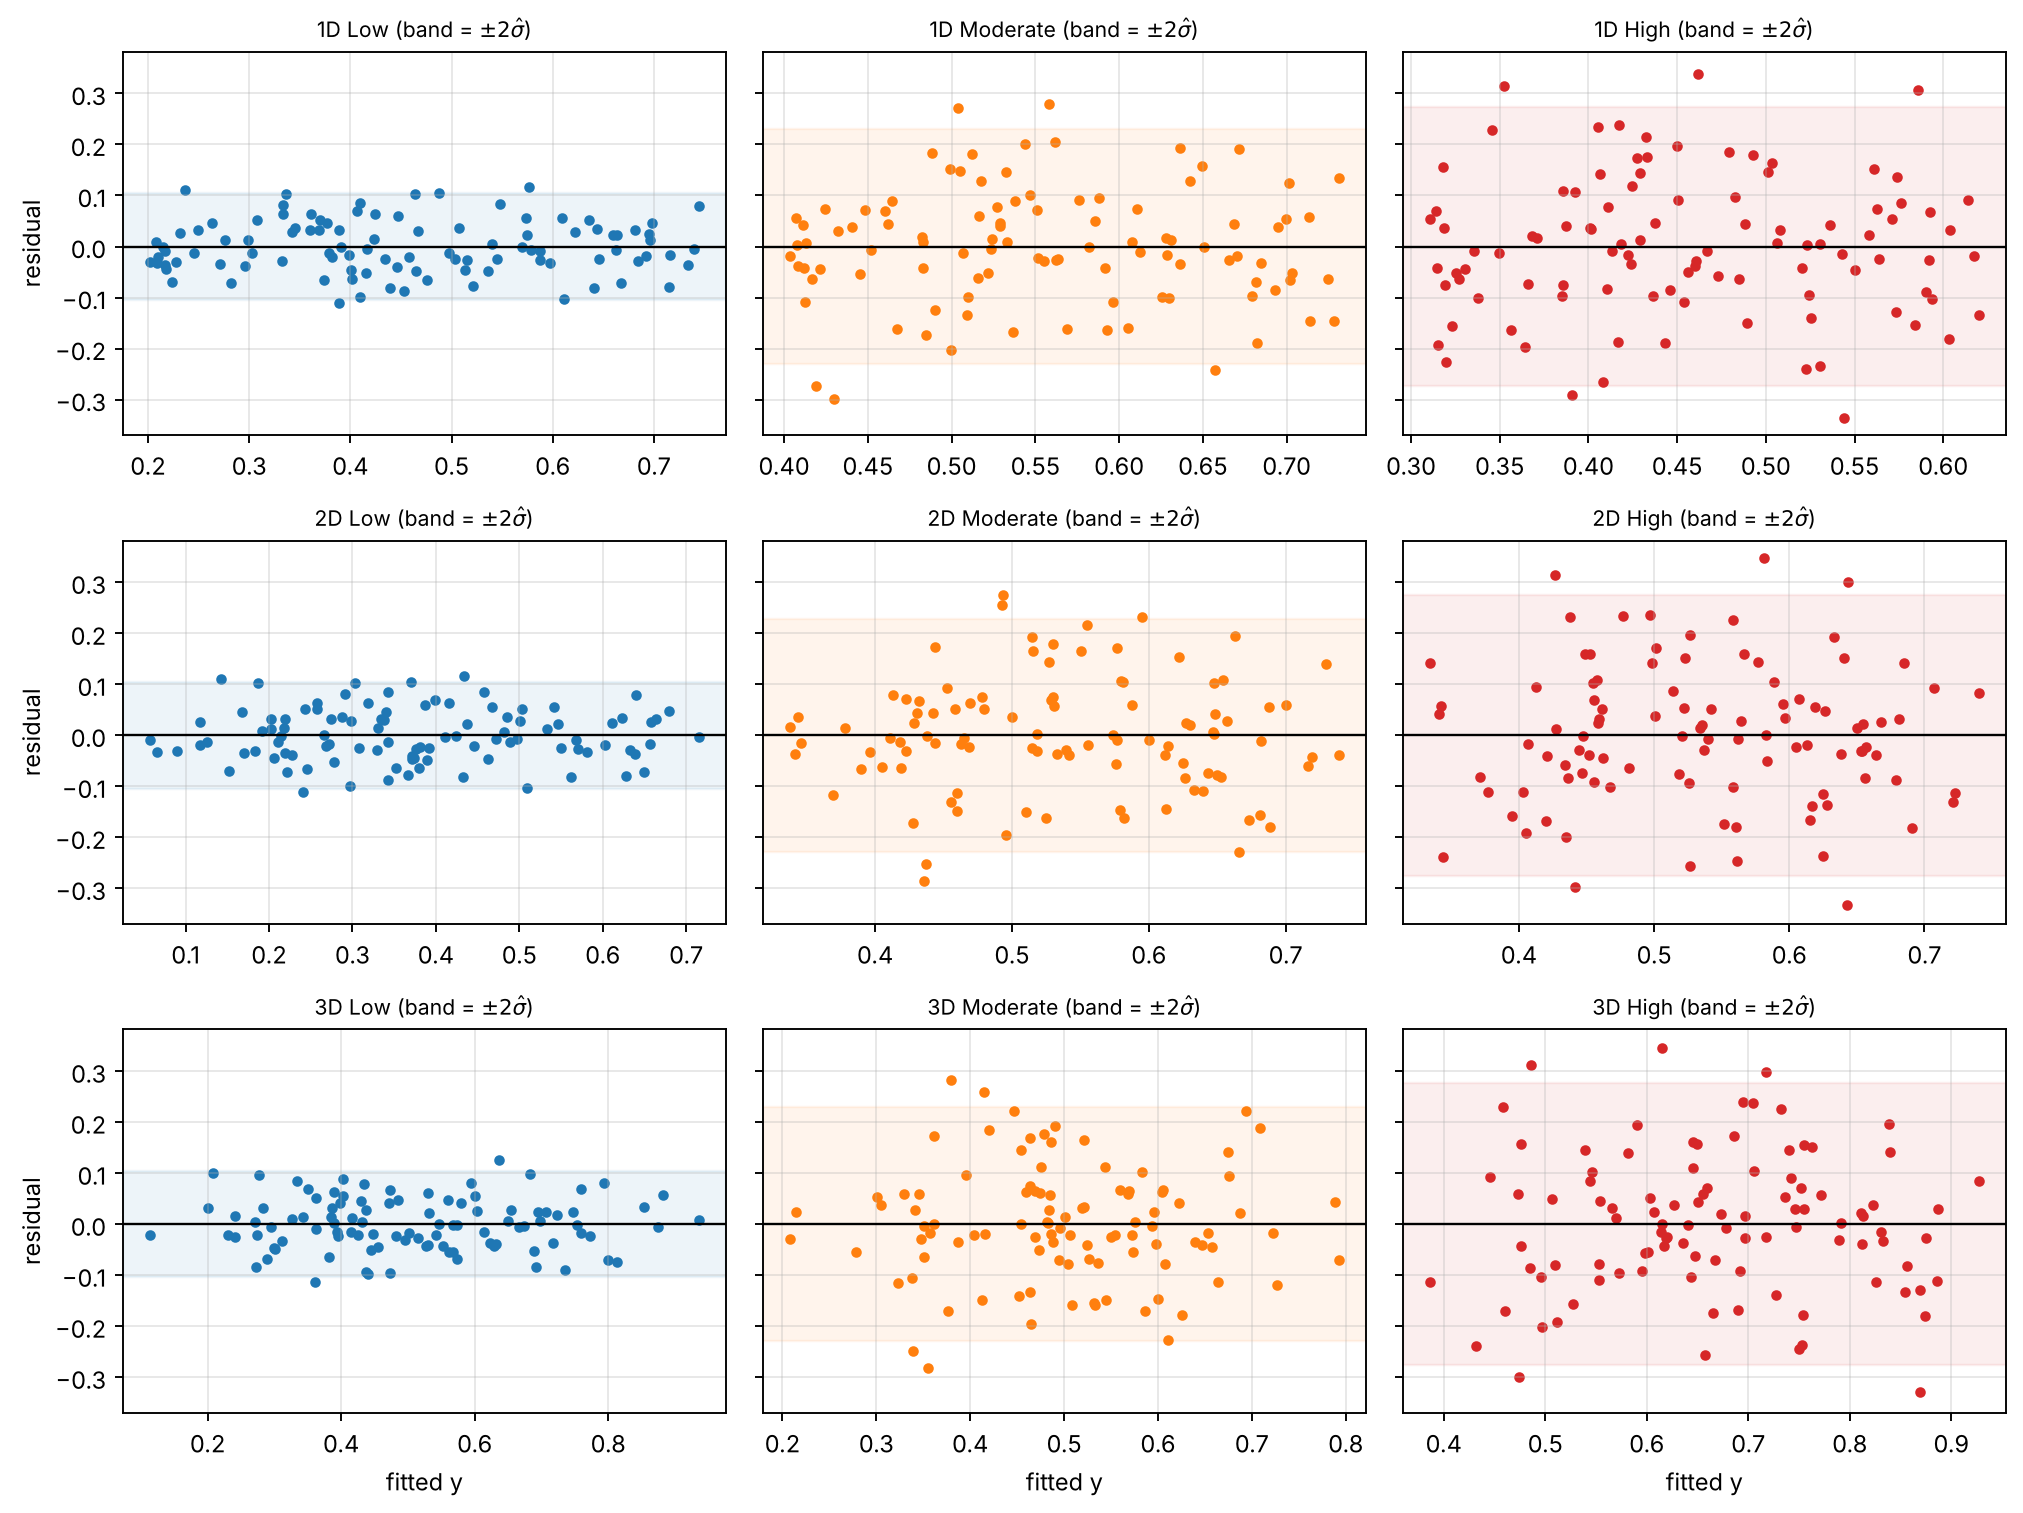
\includegraphics[width=0.92\textwidth]{../figures/fig7_residuals.png}
\caption{Residuals against fitted values. The shaded band is $\pm 2\hat\sigma$.}
\label{fig:resid}
\end{figure}

\begin{figure}[H]\centering
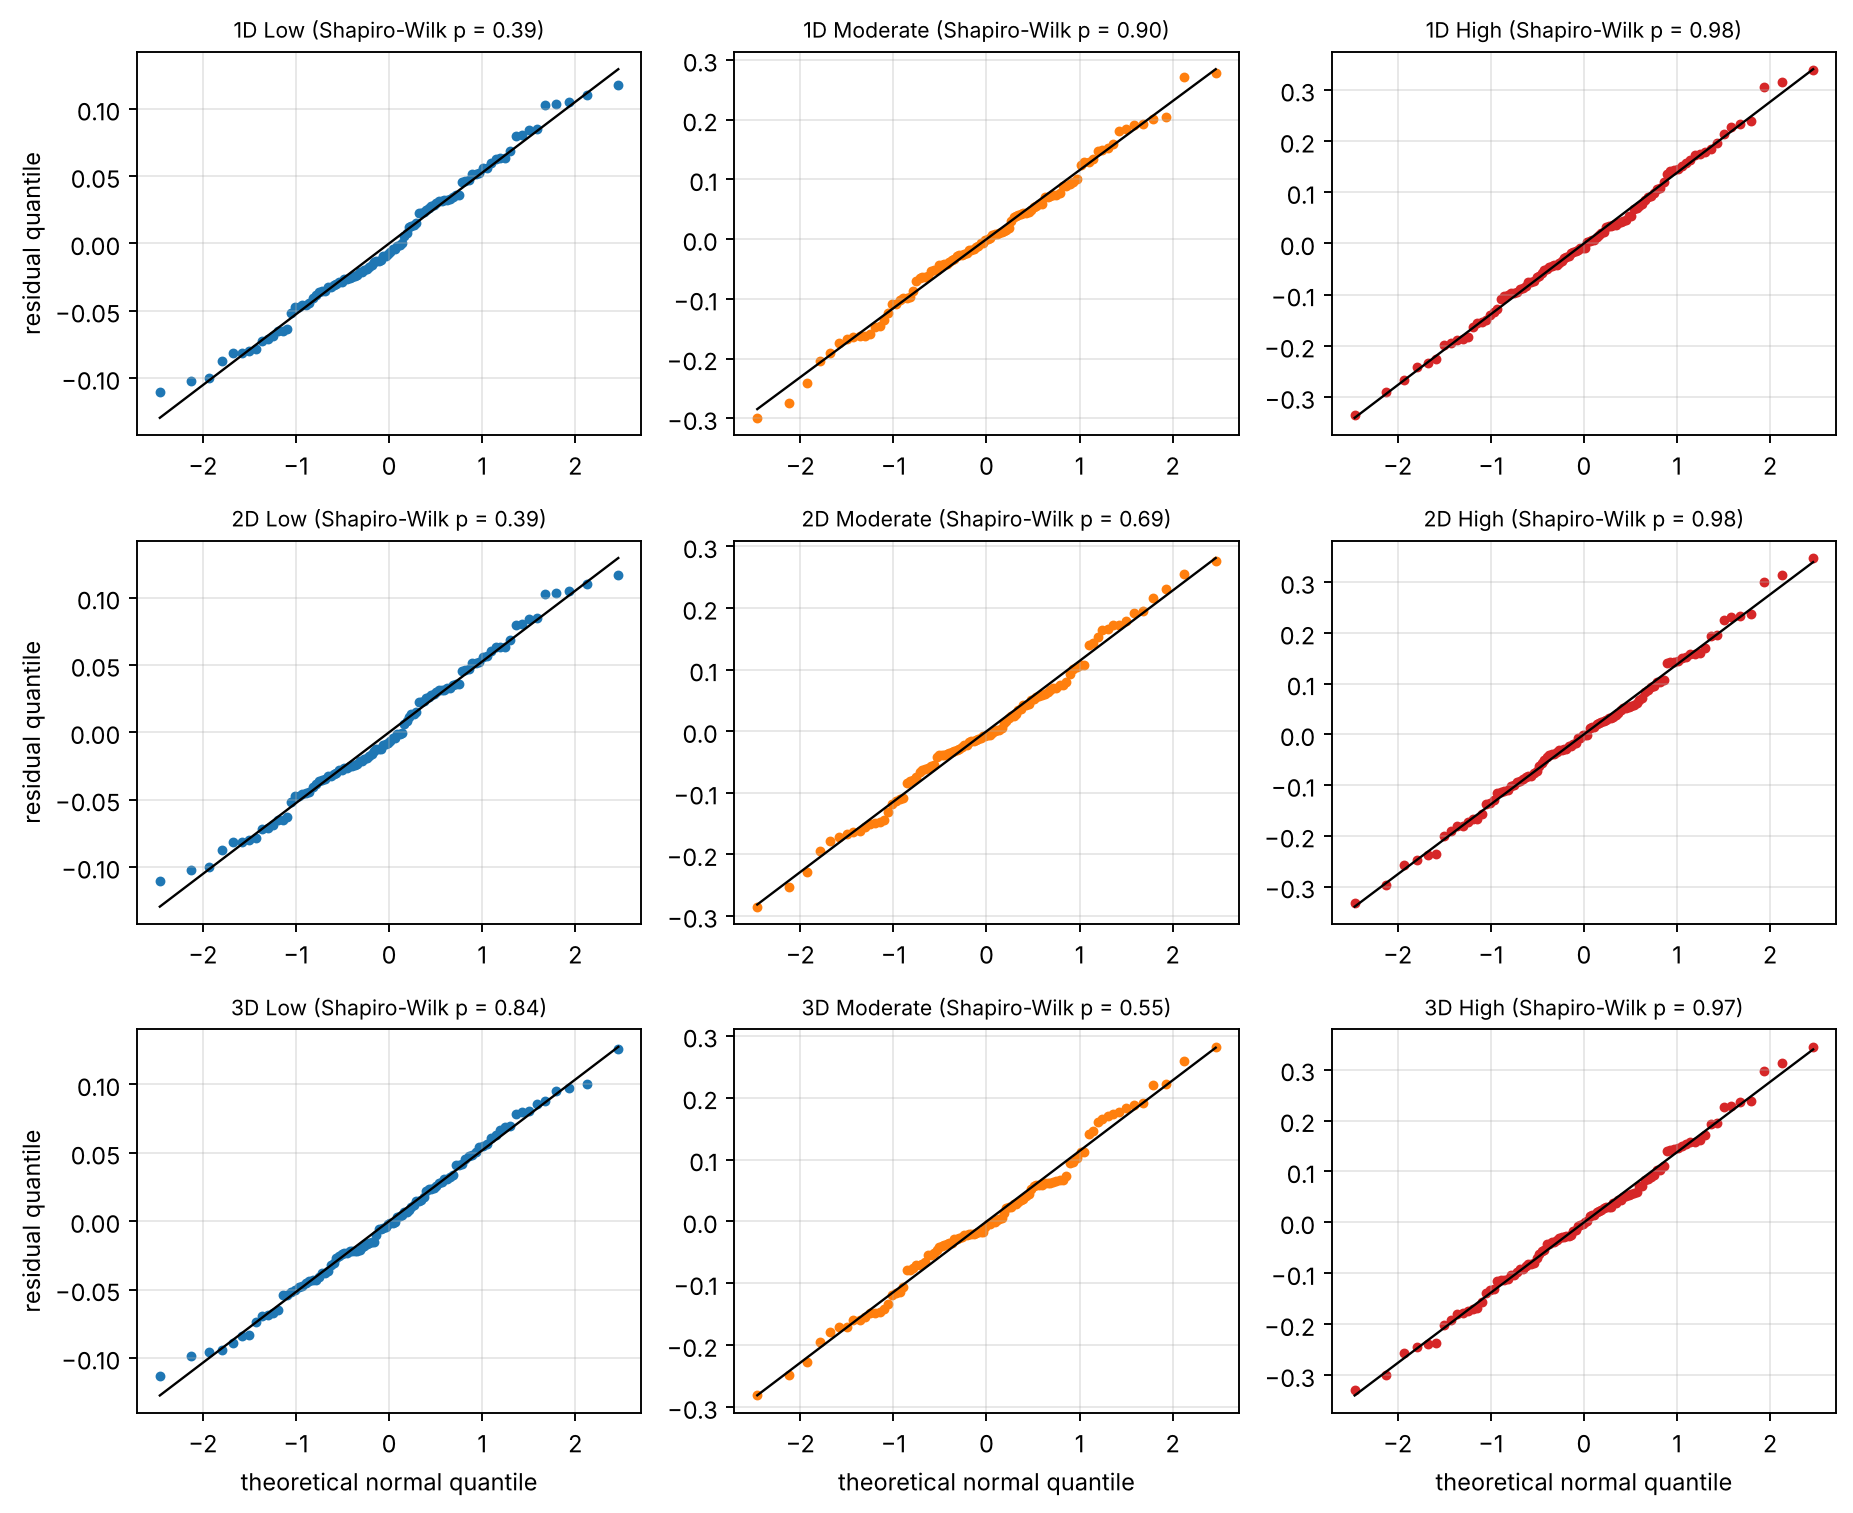
\includegraphics[width=0.86\textwidth]{../figures/fig8_qq.png}
\caption{Normal Q-Q plots of the residuals, with Shapiro-Wilk $p$-values.}
\label{fig:qq}
\end{figure}

\begin{table}[H]\centering\small
\caption{Assumption tests. Large $p$-values mean no evidence against the assumption.}
\label{tab:assump}
\begin{tabular}{lcccc}
\toprule
Dataset & Shapiro-Wilk $W$ & $p$ (normality) & Breusch-Pagan LM & $p$ (constant variance)\\
\midrule
1D Low & 0.986 & 0.39 & 0.01 & 0.90 \\
1D Moderate & 0.993 & 0.90 & 0.08 & 0.77 \\
1D High & 0.995 & 0.98 & 0.06 & 0.81 \\
\midrule
2D Low & 0.986 & 0.39 & 3.89 & 0.14 \\
2D Moderate & 0.990 & 0.69 & 3.74 & 0.15 \\
2D High & 0.995 & 0.98 & 0.10 & 0.95 \\
\midrule
3D Low & 0.992 & 0.84 & 3.71 & 0.29 \\
3D Moderate & 0.989 & 0.55 & 6.44 & 0.09 \\
3D High & 0.995 & 0.97 & 1.40 & 0.71 \\

\bottomrule
\end{tabular}
\end{table}

\subsection{Conclusions}

\begin{enumerate}[leftmargin=1.6em]
\item \textbf{Linear regression is the right model for all nine datasets.} The residuals show no structure, the assumption tests pass, and every model reaches the noise floor. No other model could predict these data much better, because what is left over is the Gaussian noise itself.
\item \textbf{Noise controls accuracy.} RMSE is set almost entirely by the noise level (about 0.051, 0.113 and 0.135), and it barely depends on the number of predictors. Higher noise also makes the coefficients less precise, with confidence intervals about 2.6 times wider at high noise than at low noise.
\item \textbf{$R^2$ must be read with the noise in mind.} An $R^2$ of 0.30 at high noise does not mean the model is poor; it means most of the variation in $y$ is unpredictable noise. RMSE compared with $\hat\sigma$, and cross-validation, are better guides to whether a model has found the true relationship.
\item \textbf{More predictors help when they carry signal.} Each added predictor raised $R^2$, adjusted $R^2$ and cross-validated $R^2$, without raising the error, because each one has a real effect. With nearly uncorrelated inputs, adding a predictor did not disturb the existing coefficients.
\item \textbf{The cost of extra parameters is small here but real.} With 100 items and at most four parameters, the train-to-test gap stays below 5\%, in line with theory. With fewer data items or many more predictors, that gap would grow, and adjusted $R^2$ or cross-validation would be needed to decide which predictors to keep.
\end{enumerate}

%=====================================================================
\section{Data organization (turned in separately)}

\begin{itemize}[leftmargin=1.4em]
\item \texttt{data/}: the nine datasets as CSV files (\texttt{1D\_L.csv} to \texttt{3D\_H.csv}), converted from the supplied PDFs without changing any value. Each has a header row; the last column is $y$.
\item \texttt{results/summary.csv}: one row per dataset with $n$, number of predictors, noise level, $R^2$, adjusted $R^2$, RMSE, MAE, $\hat\sigma$, standard deviation of $y$, the $F$ statistic and its $p$-value, cross-validated RMSE and $R^2$ (mean and standard deviation over 10 repeats), and the Shapiro-Wilk and Breusch-Pagan statistics and $p$-values.
\item \texttt{results/coefficients.csv}: one row per coefficient per dataset, with the estimate, standard error, $t$ statistic, $p$-value and 95\% confidence interval.
\item \texttt{results/equations.txt}: the nine fitted equations in plain text.
\item \texttt{results/predictions/<dataset>.csv}: for every data item, the inputs, actual $y$, fitted $\hat y$ and residual.
\item \texttt{results/verification.csv}: differences between my implementation and the two reference solvers.
\item \texttt{figures/}: every figure in this report.
\end{itemize}

%=====================================================================
\section{Credit and sources}

\paragraph{Code.} All source code is original and was written for this assignment. The OLS estimator, its inference formulas, the metrics, the Breusch-Pagan test and cross-validation follow standard textbook material \cite{islr}; the implementation is mine. NumPy provides array arithmetic, SciPy provides probability distributions and the Shapiro-Wilk test, and Matplotlib provides plotting. Scikit-learn is used only in \texttt{verify.py}, to check my results; it is not used to produce them.

\paragraph{AI assistance.} I used an AI assistant (Claude) while working on this assignment, as permitted by the course. It was used for implementation, for running the analysis, and for drafting this document. I reviewed the design choices, the results and the conclusions, and I am responsible for the content of what is submitted.

\paragraph{Data.} All nine datasets were supplied with the assignment as PDF printouts. I converted them to CSV files and renamed them to remove spaces; their values are unchanged.

\begin{thebibliography}{9}
\bibitem{islr} G. James, D. Witten, T. Hastie and R. Tibshirani, \emph{An Introduction to Statistical Learning}, 2nd ed., Springer, 2021, Chapter 3 (Linear Regression) and Chapter 5 (Resampling Methods).
\bibitem{bp} R. Koenker, ``A note on studentizing a test for heteroscedasticity,'' \emph{Journal of Econometrics}, vol. 17, no. 1, pp. 107-112, 1981.
\bibitem{sw} S. S. Shapiro and M. B. Wilk, ``An analysis of variance test for normality (complete samples),'' \emph{Biometrika}, vol. 52, no. 3/4, pp. 591-611, 1965.
\end{thebibliography}

\appendix
\section{Full coefficient inference}
\label{app:coef}
\begin{table}[H]\centering\small
\begin{tabular}{llccccc}
\toprule
Dataset & Term & Estimate & SE & $t$ & $p$ & 95\% CI\\
\midrule
1D Low & $b_0$ & 0.1982 & 0.0100 & 19.73 & $<10^{-6}$ & [0.178, 0.218] \\
 & $b_1$ & 0.5494 & 0.0184 & 29.88 & $<10^{-6}$ & [0.513, 0.586] \\
\addlinespace[2pt]
1D Moderate & $b_0$ & 0.4012 & 0.0220 & 18.20 & $<10^{-6}$ & [0.357, 0.445] \\
 & $b_1$ & 0.3318 & 0.0403 & 8.22 & $<10^{-6}$ & [0.252, 0.412] \\
\addlinespace[2pt]
1D High & $b_0$ & 0.3085 & 0.0263 & 11.72 & $<10^{-6}$ & [0.256, 0.361] \\
 & $b_1$ & 0.3133 & 0.0482 & 6.50 & $<10^{-6}$ & [0.218, 0.409] \\
\addlinespace[2pt]
2D Low & $b_0$ & 0.1980 & 0.0130 & 15.19 & $<10^{-6}$ & [0.172, 0.224] \\
 & $b_1$ & 0.5494 & 0.0185 & 29.68 & $<10^{-6}$ & [0.513, 0.586] \\
 & $b_2$ & -0.1665 & 0.0180 & -9.23 & $<10^{-6}$ & [-0.202, -0.131] \\
\addlinespace[2pt]
2D Moderate & $b_0$ & 0.3266 & 0.0283 & 11.55 & $<10^{-6}$ & [0.270, 0.383] \\
 & $b_1$ & 0.3348 & 0.0402 & 8.33 & $<10^{-6}$ & [0.255, 0.415] \\
 & $b_2$ & 0.1113 & 0.0392 & 2.84 & 0.0054 & [0.034, 0.189] \\
\addlinespace[2pt]
2D High & $b_0$ & 0.3235 & 0.0341 & 9.50 & $<10^{-6}$ & [0.256, 0.391] \\
 & $b_1$ & 0.3151 & 0.0484 & 6.51 & $<10^{-6}$ & [0.219, 0.411] \\
 & $b_2$ & 0.1342 & 0.0471 & 2.85 & 0.0054 & [0.041, 0.228] \\
\addlinespace[2pt]
3D Low & $b_0$ & 0.2144 & 0.0156 & 13.76 & $<10^{-6}$ & [0.183, 0.245] \\
 & $b_1$ & 0.5528 & 0.0184 & 30.09 & $<10^{-6}$ & [0.516, 0.589] \\
 & $b_2$ & -0.1648 & 0.0178 & -9.24 & $<10^{-6}$ & [-0.200, -0.129] \\
 & $b_3$ & 0.2144 & 0.0185 & 11.56 & $<10^{-6}$ & [0.178, 0.251] \\
\addlinespace[2pt]
3D Moderate & $b_0$ & 0.4361 & 0.0344 & 12.68 & $<10^{-6}$ & [0.368, 0.504] \\
 & $b_1$ & 0.3368 & 0.0406 & 8.30 & $<10^{-6}$ & [0.256, 0.417] \\
 & $b_2$ & 0.1123 & 0.0394 & 2.85 & 0.0053 & [0.034, 0.190] \\
 & $b_3$ & -0.2689 & 0.0409 & -6.57 & $<10^{-6}$ & [-0.350, -0.188] \\
\addlinespace[2pt]
3D High & $b_0$ & 0.3268 & 0.0415 & 7.88 & $<10^{-6}$ & [0.245, 0.409] \\
 & $b_1$ & 0.3158 & 0.0489 & 6.46 & $<10^{-6}$ & [0.219, 0.413] \\
 & $b_2$ & 0.1345 & 0.0474 & 2.84 & 0.0056 & [0.040, 0.229] \\
 & $b_3$ & 0.2319 & 0.0493 & 4.70 & 0.0000 & [0.134, 0.330] \\

\bottomrule
\end{tabular}
\end{table}

\end{document}
